\def\SigleNumero{STT-1900}
\def\NomCours{Méthodes statistiques pour l'ingénierie}
\def\DateEvaluation{1er mars 2026}
\def\HeureEvaluation{13h30 à 16h20}
\def\Session{}
\def\NomEvaluation{Examen 1}
\def\Ponderation{45}
% Ne rien mettre entre les accolades si l'enseignant (ou l'enseignante) est aussi le coordonnateur (ou la coordonnatrice)
\def\Coordonnatrice{}
\def\Coordonnateur{}

% Ne rien mettre entre les accolades s'il y a plus d'une section
\def\Enseignant{Julien Miron}
\def\Enseignante{}

% Ne rien mettre entre les accolades s'il s'agit d'un cours à section unique
% Mettre le nom de chacun des enseignants et enseignantes entre les accolades
% Une case à cocher sera générée pour chacune des sections
\def\SectionA{}
\def\SectionB{}
\def\SectionC{}
\def\SectionD{}

\newcommand{\affichepoints}{}     % ← AVEC points
% \renewcommand{\affichepoints}{on} % ← SANS points (non vide)

\def\Directives{
\begin{enumerate}
\item Matériel autorisé:
\begin{itemize}
\item Calculatrice scientifique {\bf autorisée par la faculté des sciences et de génie};
\item Votre aide-mémoire d'une feuille recto-verso, écrit à la main.
\end{itemize}
\item Assurez-vous que cette évaluation comporte \numquestions ~exercices répartis sur \numpages{}~pages, pour un total de \numpoints{}~points.\
\item \textbf{Veuillez ne pas dégrafer votre examen.}
\item Vous devez\textbf{ justifier toutes vos réponses} par une démarche claire, sauf pour les questions à choix de réponse.\
\item Pour les questions à choix de réponse et les vrais ou faux, vous pouvez mettre un X, un crochet ($\checkmark$) ou remplir la case.\
\item Vous devez laisser tout ce qui ne servira pas durant l'examen à l'avant de la salle AVANT de rejoindre votre place.\
\item Vous n'avez droit à AUCUN appareil électronique en votre possession durant l'examen.
\item Une fois assis à votre place, vous devez demandez l'autorisation pour vous lever, même si l'examen n'est pas encore commencé.
\item Dans les 5 dernières minutes de l'examen, il sera interdit de se lever avant que TOUTES les copies n'aient été ramassées.
\end{enumerate}
\begin{itemize}
\item[$\rightarrow$] Le non-respect des consignes 7-8-9 entraînera une pénalité de 10\%.
\end{itemize}
}



\documentclass{Evaluation}
\usepackage{multicol,graphicx}

\noprintanswers

\begin{document}

\pageblanche
%%%%%%%%%%%%%%%% QUESTION %%%%%%%%%%%%%%%%
\begin{questions}
\question[3]
\noindent
\begin{minipage}[t]{0.5\linewidth}\vspace{0pt}
Soit l'histogramme ci-contre.\\[0.5em]

Dans quelle classe de l'histogramme se situe le quantile d'ordre 0,30?

\begin{checkboxes}
  \choice Dans la classe [10,15[
  \correctchoice Dans la classe [15,20[
  \choice Dans la classe [20,25[
  \choice Dans la classe [25,30[
  \choice Dans la classe [30,35[
\end{checkboxes}
\end{minipage}\hfill
\begin{minipage}[t]{0.42\linewidth}\vspace{0pt}
\centering
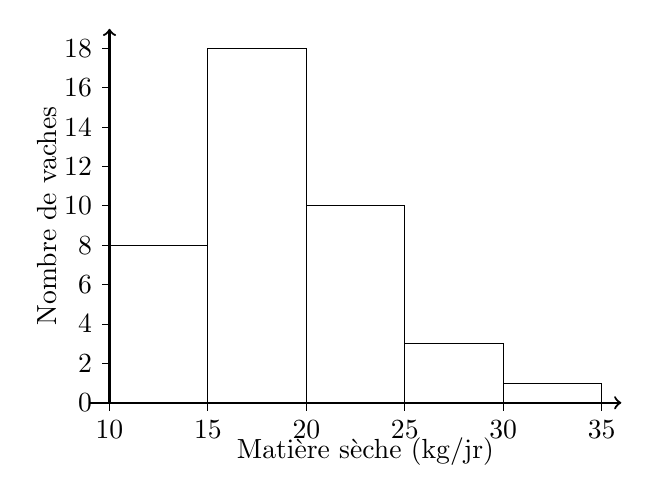
\begin{tikzpicture}[x=0.25cm,y=0.25cm]

% -------------------------------------------------
% Axes
% -------------------------------------------------
\draw[->, thick] (9,0) -- (36,0);   % axe x
\draw[->, thick] (10,0) -- (10,19); % axe y

% -------------------------------------------------
% Graduations x
% -------------------------------------------------
\foreach \x in {10,15,20,25,30,35}
  \draw (\x,0) -- (\x,-0.4) node[below] {\x};

% -------------------------------------------------
% Graduations y
% -------------------------------------------------
\foreach \y in {0,2,4,6,8,10,12,14,16,18}
  \draw (10,\y) -- (9.6,\y) node[left] {\y};

% -------------------------------------------------
% Labels
% -------------------------------------------------
\node at (23,-2.5) {Mati\`ere s\`eche (kg/jr)};
\node[rotate=90] at (6.8,9.5) {Nombre de vaches};

% -------------------------------------------------
% Histogramme
% -------------------------------------------------
\draw (10,0) rectangle (15,8);
\draw (15,0) rectangle (20,18);
\draw (20,0) rectangle (25,10);
\draw (25,0) rectangle (30,3);
\draw (30,0) rectangle (35,1);

\end{tikzpicture}
\end{minipage}

\begin{solution}
    Le nombre total de vaches est $8+18+10+3+1=40$. Le quantile d'ordre $0{,}30$ correspond à la position $0{,}30 \times 40 = 12$. L'effectif cumulé après la classe $[10,15[$ est $8$. L'effectif cumulé après la classe $[15,20[$ est $8+18=26$. Puisque $8 < 12 \leq 26$, le quantile d'ordre $0{,}30$ se situe dans la classe $[15,20[$.
\end{solution}

\vspace{0.3cm}

\question[] Dites si chaque énoncé est vrai ou faux.

\begin{parts}
    \part[1] La somme des probabilités de deux événements mutuellement exclusifs peut être plus grande que 1.
    \begin{oneparcheckboxes}
        \choice Vrai
        \correctchoice Faux
    \end{oneparcheckboxes}

    \part[1] La somme des probabilités de deux événements qui ne sont pas mutuellement exclusifs peut être plus grande que 1.

        \begin{oneparcheckboxes}
        \correctchoice Vrai
        \choice Faux
    \end{oneparcheckboxes}

        \part[1] Si la somme des probabilités de deux événements égale 1, nous savons qu'il n'y a aucune autre possibilité que ces deux événements.

        \begin{oneparcheckboxes}
        \choice Vrai
        \correctchoice Faux
    \end{oneparcheckboxes}

        \part[1] Un événement n'est pas nécessairement mutuellement exclusif avec son complément.

        \begin{oneparcheckboxes}
        \choice Vrai
        \correctchoice Faux
    \end{oneparcheckboxes}
\end{parts}


\vspace{0.3cm}
\question On a noté la fréquence cardiaque de neuf hommes. 
L'intervalle de confiance à 90\% obtenu pour la fréquence cardiaque moyenne est $[94; 112]$.
On suppose que la loi normale est adéquate pour cette variable aléatoire.


\begin{parts}
\part[1] On a confiance à 90\% que cet intervalle contient la vrai valeur moyenne de la fréquence cardiaque. 

\begin{oneparcheckboxes}
    \correctchoice Vrai
    \choice Faux
\end{oneparcheckboxes}

\begin{solution}
    Vrai. C'est l'interprétation correcte d'un intervalle de confiance: on a confiance au niveau 90\% que l'intervalle construit contient la vraie valeur du paramètre $\mu$.
\end{solution}

    \part[1] La fréquence cardiaque moyenne des hommes ayant participé à l'étude est de 100 battements par minute.
    
    \begin{oneparcheckboxes}
        \choice Vrai
        \correctchoice Faux
    \end{oneparcheckboxes}

    \begin{solution}
        Faux. L'intervalle de confiance est symétrique autour de $\bar{x}$. Donc $\bar{x}=(94+112)/2=103$, et non $100$.
    \end{solution}

    \part[1] Si on recommençait la même expérience avec neuf autres individus de la même population, il y aurait 90\% de chances que la nouvelle moyenne échantillonnale soit comprise entre 94 et 112.
    
    \begin{oneparcheckboxes}
        \choice Vrai
        \correctchoice Faux
    \end{oneparcheckboxes}

    \begin{solution}
        Faux. L'intervalle de confiance ne prédit pas la valeur d'une future moyenne échantillonnale. Le niveau de confiance de 90\% signifie que la procédure de construction de l'intervalle capture $\mu$ dans 90\% des cas.
    \end{solution}

    \part[1] Environ 90\% des hommes de cette population ont une fréquence cardiaque comprise entre 94 et 112.
    
    \begin{oneparcheckboxes}
        \choice Vrai
        \correctchoice Faux
    \end{oneparcheckboxes}

    \begin{solution}
        Faux. L'intervalle de confiance est construit pour la moyenne $\mu$, pas pour les valeurs individuelles de la population.
    \end{solution}

        \part[1] Environ 90\% des hommes de cet échantillon ont une fréquence cardiaque comprise entre 94 et 112.
    
    \begin{oneparcheckboxes}
        \choice Vrai
        \correctchoice Faux
    \end{oneparcheckboxes}

    \begin{solution}
        Faux. L'intervalle de confiance ne porte pas sur la proportion d'individus de l'échantillon dans un intervalle, mais bien sur la localisation de la moyenne $\mu$.
    \end{solution}
    
\end{parts}

\vspace{0.3cm}

\pageblanche
\question[4] Laquelle des fonctions suivantes est une fonction de répartition?


\begin{checkboxes}
\choice $F(a)=a,\ \mbox{si } 0 <a$
		
\correctchoice $ F(b) = \left\{
			\begin{array}{ll}
			0  & \mbox{ si } b<0, \\
			b & \mbox{ si } 0\leq b < 1,\\
			1 & \mbox{ si } 1 \leq b
			\end{array}
			\right. $
\choice $ F(c) = \left\{
			\begin{array}{ll}
			\sqrt{c}  & \mbox{ si } 0\leq c\leq 1, \\
			0 & \mbox{sinon}
			\end{array}
			\right. $
\choice $ F(d) = \left\{
			\begin{array}{ll}
			0  & \mbox{ si } d < -1, \\
			|d| & \mbox{ si } -1 \leq d \leq 1,\\
			1 &  \mbox{ si } 1 < d
			\end{array}
			\right. $
\end{checkboxes}

\question[6]
Dans un laboratoire de microtechnique, Benjamin et Guillaume ont étudié le temps de réaction (en millisecondes) d'un certain type de détecteur de mouvements. Les 21 valeurs suivantes sont des temps de réaction collectés au cours d'une journée:

\begin{center}
\begin{tabular}{  c c c c c c c c }
111  &111  &111  &112  &113  &113  &113 \\
113 &115  &115  &115  &115 &115 & 116 \\
116 & 118 & 118 & 119 & 125 &125 & 128\\
\end{tabular}
\end{center}

Le diagramme en boîte ci-dessous a été tracé à partir de ces résultats. Il manque toutefois quelque chose à ce diagramme (il ne s'agit pas d'un titre ou de noms d'axes).


Ajoutez \textbf{sur le diagramme} l'élément manquant et dites ce que vous avez fait sous le diagramme. Un ajout sur le diagramme sans justification n'aura aucun point.
\begin{center}
		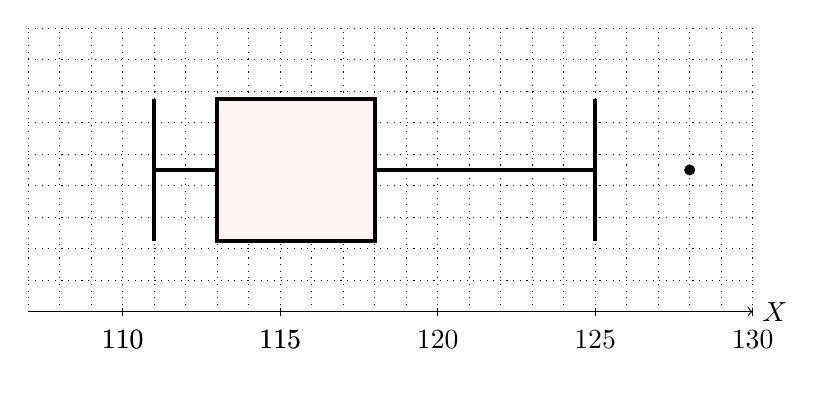
\begin{tikzpicture}[x=0.4cm,y=0.9cm]
         \draw[step=0.4cm,,dotted,color=black] (107,0) grid (130,4);
		\draw[->] (107,0) -- (130,0) node[right] {$X$} ;
		\foreach \X in {110,115,110,115,120,125,130} {
			\draw (\X,0.05cm) -- (\X,-0.05cm) node[below] {$\X\strut$};}
		\draw[ultra thick][fill=red!5] (113,1) rectangle (118,3);


		\draw[ultra thick] (111,1) -- (111,3);
		\draw[ultra thick] (111,2) -- (113,2);
		\draw[ultra thick] (118,2) -- (125,2);
		%\draw[ultra thick] (4,1) -- (4,3);
		\draw[ultra thick] (125,1) -- (125,3);
        \node[circle, fill=black, inner sep=0pt, minimum size=4pt] at (128,2) {};
			\end{tikzpicture}\\
	\end{center}

\begin{solution}
    Il manque la ligne de la médiane dans le diagramme en boîte. Les 21 données ordonnées donnent une médiane égale à la 11\textsuperscript{e} valeur, soit $\tilde{x}=115$. Il faut donc tracer un trait vertical à $x=115$ à l'intérieur de la boîte.

    On vérifie les autres éléments:
    \begin{itemize}
        \item $Q_1 = (x_{(5)}+x_{(6)})/2=(113+113)/2=113$ \checkmark
        \item $Q_3 = (x_{(16)}+x_{(17)})/2=(118+118)/2=118$ \checkmark
        \item $\text{IQR}=Q_3 - Q_1 = 5$
        \item Barrière supérieure: $Q_3+1{,}5\times\text{IQR}=118+7{,}5=125{,}5$
        \item La valeur $128 > 125{,}5$ est une valeur aberrante, correctement représentée par un point. \checkmark
        \item La moustache supérieure s'arrête à $125$, la plus grande valeur non aberrante. \checkmark
        \item La moustache inférieure s'arrête à $111$, la plus petite valeur. \checkmark
    \end{itemize}
\end{solution}

\pageblanche

\question Un sac contient 40 dés rouges, 40 dés verts et 20 dés bleus.
Les dés rouges et les dés verts sont numérotées de <<1>> à <<6>>.
Les dés bleus ont 6 fois la face <<1>>.

L'expérience aléatoire consiste à choisir un dé dans le sac, à le lancer et à noter la face du dessus.

Pour répondre aux questions, utilisez $\mathcal{S}$ pour désigner l'espace échantillonnal et les événements suivants:

\begin{itemize}
    \item R: le dé choisi est rouge,
    \item V: le dé choisi est vert,
    \item B: le dé choisi est bleu,
    \item U: la face sur le dessus du dé lancé est <<1>>,
    \item D: la face sur le dessus du dé lancé est <<2>>.
\end{itemize}

\begin{parts}
    \part[7] La face sur le dessus du dé lancé est <<1>>. Quelle est la probabilité que le dé lancé soit rouge?


\begin{solution}
    On sait que $P(R)=0,4$, $P(V)=0,4$, $P(B)=0,2$ $P(N|R)=P(N|V)=1/6$, $P(N|B)=1$. On peut déduire que 

    \begin{align*}
        P(N)&=P(N\cap R)+P(N\cap V)+P(N\cap B)\\
        &= P(N|R)P(R)+P(N|V)P(V)+P(N|B)P(B)\\
        &=\frac{1}{6}\times 0,4+\frac{1}{6}\times 0,4 + 0,4 \times 1\\
        &=\displaystyle\frac{8}{15}
    \end{align*}

    On cherche $P(R|N)$.

    \begin{align*}
        P(R|N)&=\frac{P(N\cap R)}{P(N)}\\
        &=\frac{P(N|R)P(R)}{P(N)}\\
        &= \frac{\sfrac{1}{6}\times 0,4}{\sfrac{8}{15}}\\
        &=\frac{1}{8}
    \end{align*}
\end{solution}

\vspace{14cm}

\part[3] Les événements $B$ et $D$ sont-ils indépendants? \textit{Justifiez votre réponse.}

\begin{oneparcheckboxes}
    \choice Oui
    \correctchoice Non
\end{oneparcheckboxes}

\begin{solution}
    \begin{itemize}
        \item $R$ et $B$ ne sont pas indépendants car $P(R \cap B)=0 \neq P(R)P(B)=0{,}4\times0{,}2=0{,}08$.
        \item $R$ et $B$ sont mutuellement exclusifs car un dé ne peut pas être à la fois rouge et bleu, donc $P(R \cap B)=0$.
        \item $B$ et $U$ ne sont pas indépendants car $P(B \cap U)=P(U|B)P(B)=1\times 0{,}2=0{,}2$ alors que $P(B)P(U)=0{,}2\times\sfrac{8}{15}=\sfrac{4}{75}\neq 0{,}2$.
        \item $B$ et $U$ ne sont pas mutuellement exclusifs car $P(B \cap U)=0{,}2\neq 0$.
    \end{itemize}
\end{solution}

\end{parts}


\pageblanche

\question\label{densite} Soit $X$ une variable aléatoire continue de densité $f_X$ définie ci-dessous.

\begin{minipage}[]{7cm}{
\vspace{0cm}
\[ f_X(x) = \begin{cases}
\vspace{0.2cm}
\displaystyle \frac{1}{18} & \mbox{si } 0\leq x < \displaystyle \frac{a}{5}, \\
\vspace{0.2cm}
\displaystyle \frac{1}{9} & \mbox{si } \displaystyle\frac{a}{5}\leq x \leq \displaystyle a, \\
\displaystyle 0 & \mbox{sinon.}
\end{cases} \]
    }
\end{minipage}
 \hspace{10mm}
\begin{minipage}[]{7cm}{
\vspace{0cm}
\begin{tikzpicture}[xscale=0.6, yscale=25]

% Axes
\draw[->, thick] (-1,0) -- (11.8,0) node[right] {$x$};
\draw[->, thick] (0,-0.002) -- (0,0.14) node[above] {$f_X(x)$};

% Graduations x
  \draw (2,0) -- (2,-0.002) node[below] {$\displaystyle \Large
  \sfrac{a}{5}$};
    \draw (10,0) -- (10,-0.002) node[below] {$\displaystyle 
  a$};

% Niveaux y
\draw (-0.15,1/18) -- (0,1/18) node[left] { $\frac{1}{18}$};
\draw (-0.15,1/9)  -- (0,1/9)  node[left] {$\frac{1}{9}$};

% Segments de la densité
\draw[very thick] (-1,0) -- (0,0);
\draw[very thick] (10,0) -- (11.8,0);
\draw[very thick] (0,1/18) -- (2,1/18);
\draw[very thick] (2,1/9) -- (10,1/9);

% Points (NODES -> pas déformés par xscale/yscale)
\node[circle, draw=black, inner sep=0pt, minimum size=4pt] at (0,0) {};
\node[circle, fill=black, inner sep=0pt, minimum size=4pt] at (0,1/18) {};
\node[circle, draw=black,  inner sep=0pt, minimum size=4pt] at (2,1/18) {}; % ouvert
\node[circle, fill=black, inner sep=0pt, minimum size=4pt] at (2,1/9) {};
\node[circle, fill=black, inner sep=0pt, minimum size=4pt] at (10,1/9) {};
\node[circle, draw=black, inner sep=0pt, minimum size=4pt] at (10,0) {};

\end{tikzpicture}
    }
\end{minipage}

\begin{parts}
    \part[4] Que vaut $a$?

    \begin{solution}
        On veut que l'aire totale sous la courbe donne 1. On peut faire l'intégrale ou la somme des deux rectangles. 

        \begin{align*}
            1&=\sfrac{a}{5}\times \sfrac{1}{18}+(a-\sfrac{a}{5}\times \sfrac{1}{9}\\
            1&=\sfrac{a}{90}+\sfrac{4a}{45}\\
            1&=\frac{9a}{90}\\
            10&=a
        \end{align*}
    \end{solution}
\vspace{5cm}
    \part[6] Quelle est la probabilité que $X$ prenne une valeur entre $\displaystyle \frac{a}{10}$ et $\displaystyle \frac{a}{2}$? \textit{Si vous n'avez pas trouvé la valeur de $a$, vous pouvez donner votre réponse en fonction de $a$.}

    \begin{solution}
        On peut encore faire l'intégrale entre les deux points ou calculer l'aire des deux rectangles formés. 

        \begin{align*}
            P(\sfrac{a}{10}<X<\sfrac{a}{2})&=P(1<X<5)\\
            &=(2-1)\times \sfrac{1}{18}+(5-2)\times \sfrac{1}{9}\\
            &=\sfrac{1}{18}+\sfrac{1}{3}\\
            &= \frac{7}{18}
        \end{align*}
    \end{solution}

\end{parts}


\pageblanche



\question\label{examnormal}
L'examen A et l'examen B servent pour la classification à un même emploi. 
Nous savons que les notes de ces deux examens suivent des lois normales d'espérance $\mu_{A}=1100$ et $\mu_{B}=21$, respectivement, de variance $\sigma^2_{A}=40\ 000$ et $\sigma^2_{B}=36$, respectivement et de fonctions de répartition $F_A$ et $F_B$, respectivement.
Nous établissons le pointage d'un candidat par la probabilité d'obtenir une note inférieure ou égale à la note du candidat en question (donc en évaluant $F_A(a)$ ou $F_B(b)$, pour un candidat ayant obtenu $a$ à l'examen A ou $b$ à l'examen B). 

\vspace{0.5cm}
\begin{parts}
    \part[7] Lucie a eu une note de 1300 à l'examen A alors que Camille a eu une note de 24 à l'examen B. Laquelle des deux a un meilleur pointage?

\begin{solution}
    Note de Lucie: 

    \begin{align*}
        P(A<1300)&=\displaystyle P\left(\frac{A-1100}{200}<\frac{1300-1100}{200}\right)\\
        &= \displaystyle P\left(Z<1\right)\\
        &= 0,84134
    \end{align*}

        Note de Camille: 

    \begin{align*}
        P(B<24)&=\displaystyle P\left(\frac{B-21}{6}<\frac{24-21}{6}\right)\\
        &= \displaystyle P\left(Z<0,5\right)\\
        &= 0,69146
    \end{align*}

    Donc Lucie a la meilleure note.
\end{solution}
\vspace{12cm}
\part[5] Quelle note aurait dû avoir Lucie afin d'obtenir le même pointage que Camille?

\begin{solution}
    On doit trouver la valeur $m$ de $A$ qui donne $0,5$ une fois standardisée. Donc,

    \begin{align*}
        \frac{m-1100}{200}&=0,5\\
        m-1100&=100\\
        m&=1200
    \end{align*}
\end{solution}



\vfill
\pagesuivante{\ref{examnormal}}

    \part[6] On tente de faire accréditer l'examen C pour le même emploi. On sait que la note à l'examen~C est de loi quelconque, d'espérance $50$ et de variance $25$. 
On demande à 64 personnes de passer l'examen~C. Quelle est la probabilité que la note moyenne de ces 64 personnes soit inférieure à 51,225?

\begin{solution}
    Soit $C_1,\hdots,C_{64}$ les notes des 64 personnes. On a $E(C_i)=50$ et $V(C_i)=25$. Par le théorème central limite, puisque $n=64$ est suffisamment grand:
    $$\bar{C}=\frac{1}{64}\sum_{i=1}^{64}C_i \stackrel{\cdot}{\sim} N\left(50,\frac{25}{64}\right)$$
    Donc:
    \begin{align*}
        P(\bar{C}<51{,}225)&=P\left(Z<\frac{51{,}225-50}{\sqrt{25/64}}\right)\\
        &= P\left(Z<\frac{1{,}225}{5/8}\right)\\
        &= P(Z<1{,}96)\\
        &= 0{,}975
    \end{align*}
\end{solution}
\end{parts}

\pageblanche
\question\label{cov}

Soit $X$, $Y$ et $W$ trois variables aléatoires avec
\begin{itemize}
\item $E(X)=1$, $E(Y)=0$, $E(W)=0$
\item $V(X)=16$, $V(Y)=4$, $V(W)=25$
\item $Cov(X,Y)=-2$, $Cov(X,W)=2$ et $W$ est indépendante de $Y$.
\end{itemize}


\begin{parts}
    \part[3] Calculez $E(3+4X-Y+W)$.

    \begin{solution}
        \begin{align*}
            E(3+4X-Y+W)&= E(3)+4E(X)-E(Y)+E(W)\\
            &= 3+ 4*1-0+0\\
            &=7
        \end{align*}
    \end{solution}
\vspace{8 cm}
    \part[7] Calculez $V(3+4X-Y+W)$.

        \begin{solution}
        \begin{align*}
            V(3+4X-Y+W)&= 4^2V(X)+(-1)^2V(Y)+V(W)+2\left[Cov(4X,-Y)+Cov(4X,W)\right]\\
            &= 4^2V(X)+(-1)^2V(Y)+V(W)+2\left[-4Cov(X,Y)+4Cov(X,W)\right]\\
            &=4^2\times16+(-1)^2\times4+25+2\left[-4\times-2+4\times2\right]\\
            &=317
        \end{align*}
    \end{solution}
\end{parts}





    \pageblanche

    \question Soit $X_1,\hdots,X_5$ un échantillon de taille $n=5$ provenant d'une variable aléatoire de fonction de répartition $F_X$, d'espérance $\mu$ et de variance $\sigma^2$.

    Pour estimer $\mu$, nous voulons comparer la performance de deux estimateurs:

    \begin{align*}
        \hat{\mu}_1=\overline{X}, & & \hat{\mu}_2=0,1X_1+0,2X_2+0,2X_3+0,2X_4+0,1X_5.
    \end{align*}

    \begin{parts}
        \part[5] Lequel des deux estimateurs a la plus faible variance?
\begin{solution}
    \begin{align*}
        V(\hat{\mu}_1)&=V(\overline{X})\\
        &=\frac{\sigma^2}{5}
    \end{align*}
    \begin{align*}
        V(\hat{\mu}_2)&=V(0,1X_1+0,2X_2+0,2X_3+0,2X_4+0,1X_5)\\
        &=0,1^2V(X_1)+0,2^2V(X_2)+0,2^2V(X_3)+0,2^2V(X_4)+0,1^2V(X_5)\\
        &=0,14\sigma^2
    \end{align*}

    Donc $ V(\hat{\mu}_2)< V(\hat{\mu}_1)$.
\end{solution}
        \vspace{8cm}
        \part[7] On sait que $biais(\hat{\mu}_2,\mu)=-0,2\mu$. En supposant que $\sigma^2=1$, pour quelles valeurs de $\mu$ a-t-on que l'estimateur $\hat{\mu}_2$ est meilleur que $\hat{\mu}_1$ au niveau du MSE?

        \begin{solution}
            \begin{align*}
                MSE(\hat{\mu}_1,\mu)&=\frac{\sigma^2}{5}\\
                &= 0,2
            \end{align*}

                        \begin{align*}
                MSE(\hat{\mu}_2,\mu)&=(-0,2\mu)^2+0,14\sigma^2\\
                         &= 0,04\mu^2+0,14
            \end{align*}
            On cherche les valeurs de $\mu$ pour que $MSE(\hat{\mu}_2,\mu)<MSE(\hat{\mu}_1,\mu)$.
                      \begin{align*}
                MSE(\hat{\mu}_2,\mu)&<MSE(\hat{\mu}_1,\mu)\\
                0,04\mu^2+0,14&<0,2\\
                |\mu| &< 1,225
            \end{align*}
            
        \end{solution}
    \end{parts}

    \pageblanche


    \question[8] Soit $X_1,\hdots,X_{121}$, des variables aléatoires provenant d'une loi normale d'espérance $\mu=0$ et de variance $\sigma^2=16$. Quelle est la probabilité que $\displaystyle\frac{\overline{X}}{S}$ soit plus grand que $0,18$, où $S$ est l'écart-type échantillonnal?

    \begin{solution}
        \begin{align*}
            P\left(\frac{\overline{X}}{S}>0,18\right)&=P\left(\frac{\overline{X}}{S/\sqrt{121}}>1,98\right)\\
            &= P\left(t_{120}>1,98\right)\\
            &=0,025
        \end{align*}
    \end{solution}

    \pageblanche

    \question Soit $X_1,\hdots, X_{100}$, des variables aléatoires indépendantes et identiquement distribuées selon une loi normale d’espérance $\mu$ et de variance $\sigma^2 = 400$. 
Nous désirons construire un intervalle de confiance approprié de niveau $95\%$ pour $\mu$. Nous notons cet intervalle $[C_1;C_2]$.
\begin{parts}
    \part[3] Que vaut $\mathbb{E}[C_2]$?

    \begin{solution}
        Puisque $\sigma^2 = 400$ est connu et que les $X_i$ suivent une loi normale, l'intervalle de confiance à 95\% est:
        $$\left[\bar{X}-z_{0{,}025}\frac{\sigma}{\sqrt{n}}\;;\;\bar{X}+z_{0{,}025}\frac{\sigma}{\sqrt{n}}\right]=\left[\bar{X}-1{,}96\times\frac{20}{10}\;;\;\bar{X}+1{,}96\times\frac{20}{10}\right]$$
        Donc $C_1=\bar{X}-3{,}92$ et $C_2=\bar{X}+3{,}92$.
        \begin{align*}
            E(C_2)&=E(\bar{X}+3{,}92)\\
            &= E(\bar{X})+3{,}92\\
            &= \mu + 3{,}92
        \end{align*}
    \end{solution}
    \vspace{7cm}
    \part[3] Que vaut $\text{Var}[C_2]$?

    \begin{solution}
        \begin{align*}
            \text{Var}(C_2)&=\text{Var}(\bar{X}+3{,}92)\\
            &= \text{Var}(\bar{X})\\
            &= \frac{\sigma^2}{n}=\frac{400}{100}=4
        \end{align*}
    \end{solution}
    \vspace{7cm}

    \part[4]Quelle est la probabilité que $C_2$ soit inférieure ou égale à $\mu$? 

    \begin{solution}
        \begin{align*}
            P(C_2\leq \mu)&=P(\bar{X}+3{,}92\leq \mu)\\
            &= P\left(\frac{\bar{X}-\mu}{\sigma/\sqrt{n}}\leq \frac{-3{,}92}{20/10}\right)\\
            &= P(Z\leq -1{,}96)\\
            &= 0{,}025
        \end{align*}
    \end{solution}




\end{parts}
\end{questions}

\end{document} 
